\documentclass[../main.tex]{subfiles}

\begin{document}
	\section{General Wave Properties}
	\begin{preamb}
		Waves are a fundamental method of describing the nature of matter and how it interacts with energy. In this chapter we will be covering general wave properties that would be helpful.
	\end{preamb}
	
	\subsection{Definitions}
	\pdef{Wave}{A wave is made up of periodic motion. A wave is a disturbance that transfers energy from one place to another without transfer of matter.}
	
	\pdef{Transverse Wave}{A transverse wave is when the particles oscillate perpendicular to the direction of propagation.}
	An example of a transverse wave is electromagnetic waves.
	
	\begin{center}
		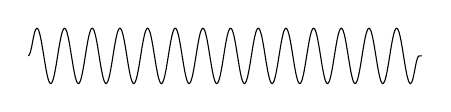
\begin{tikzpicture}
			\draw[decorate, decoration={snake, segment length=10, amplitude=10}] (0,0) -- (5,0);
		\end{tikzpicture}
	\end{center}
	
	\pdef{Longitudinal Wave}{A longitudinal wave is when the particles oscillate parallel to the direction of propagation.}
	An example of a longitudinal wave is sound waves.
	
	\begin{center}
		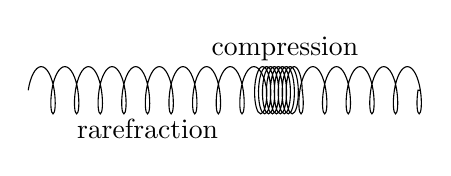
\begin{tikzpicture}
			\draw[decorate, decoration={coil, aspect=0.3, segment length=3mm, amplitude=3mm}] (0,0) --(3.03,0)node[pos=0.5, anchor=north, yshift = -2.5mm] {rarefraction};
			\draw[decorate, decoration={coil, aspect=0.3, segment length=0.5mm, amplitude=-3mm}] (3.03,0) -- (3.49,0) node[pos=0.5, anchor=south, yshift = 2.5mm] {compression}; 
			\draw[decorate, decoration={coil, aspect=0.3, segment length=3mm, amplitude=-3mm}] (3.48,0) -- (4.98,0);
		\end{tikzpicture}
	\end{center}
	
	\subsection{Parts of a Wave}
	
	\subsubsection{Common Quantities}
	\pdef{Amplitude}{The amplitude of a wave is the maximum displacement of a particle in a wave. It is usually represented by the letter \(A\). The most common unit for amplitude is the metre [\si{\meter}]; though keep in mind other physical quantities like voltage can exhibit periodic wave-like behaviour.}
	
	\pdef{Wavelength}{The wavelength of a wave is the displacement between two successive in-phase points. It is usually represented by the Greek letter \(\lambda\). The SI unit for wavelength is the metre [\si{\meter}].}
	
	\pdef{Wavefront}{A wavefront is an imaginary line on a wave that joins all adjacent points that are in phase.}
	
	\subsubsection{Time-based Quantities}
	\pdef{Period}{The period of a wave is the time taken for a particle to complete one oscillation. It is usually represented by the letter \(T\). The SI unit for period is the second [\si{\second}].}
	
	\pdef{Frequency}{The frequency of a wave is the number of times a particle completes one oscillation in one second. It is usually represented by the letter \(f\). The SI unit for frequency is the hertz [\si{\hertz}].}
	
	\peqn{Period and Frequency}{Period and frequency are reciprocals of each other,}{f = \frac{1}{T} \Leftrightarrow T = \frac{1}{f}}
	
	\subsubsection{Some Things Specific to Longitudinal Waves}
	\pdef{Compression}{A compression in a longitudinal wave is where there are more particles around that region than in equilibrium.}
	\pdef{Rarefaction}{A rarefaction in a longitudinal wave is where there are less particles around that region than in equilibrium.}
	
	\subsection{Graphs}
	\subsubsection{Displacement-distance Graph}
	This is also known as a snapshot graph.
	\begin{center}
		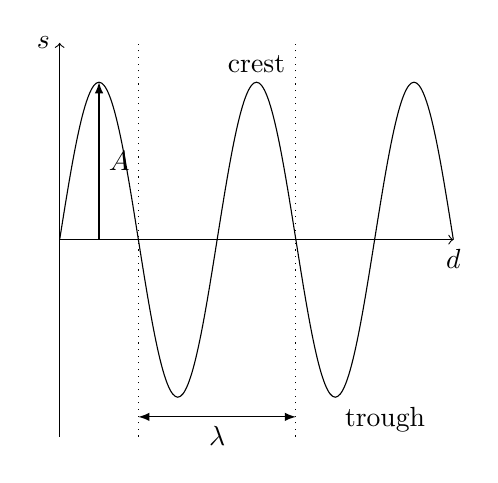
\begin{tikzpicture}
			\draw [->] (0,-2.5) -- (0,2.5) node [anchor=east] {\(s\)};
			\draw [->] (0,0) -- (5,0) node [anchor=north] {\(d\)};
			\draw (0,0) sin (0.5,2) cos (1,0) sin (1.5,-2)cos (2,0) sin (2.5,2) node [anchor=south] {crest} cos (3,0) sin (3.5,-2) node [anchor=north west] {trough} cos (4,0) sin (4.5,2) cos (5,0);
			\draw [-latex] (0.5,0) -- (0.5,2) node [pos=0.5, anchor=west] {\(A\)};
			\draw [dotted] (1, -2.5) -- (1, 2.5);
			\draw [dotted] (3, -2.5) -- (3, 2.5);
			\draw [latex-latex] (1, -2.25) -- (3, -2.25) node [pos=0.5, anchor=north] {\(\lambda\)};
		\end{tikzpicture}
	\end{center}
	
	\subsubsection{Displacement-time Graph}
	This is also known as a history graph.
	\begin{center}
		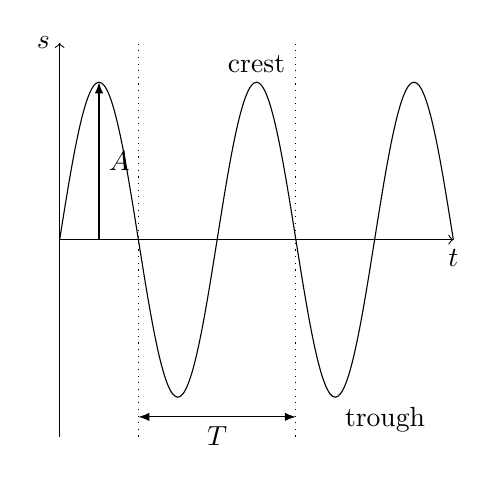
\begin{tikzpicture}
			\draw [->] (0,-2.5) -- (0,2.5) node [anchor=east] {\(s\)};
			\draw [->] (0,0) -- (5,0) node [anchor=north] {\(t\)};
			\draw (0,0) sin (0.5,2) cos (1,0) sin (1.5,-2)cos (2,0) sin (2.5,2) node [anchor=south] {crest} cos (3,0) sin (3.5,-2) node [anchor=north west] {trough} cos (4,0) sin (4.5,2) cos (5,0);
			\draw [-latex] (0.5,0) -- (0.5,2) node [pos=0.5, anchor=west] {\(A\)};
			\draw [dotted] (1, -2.5) -- (1, 2.5);
			\draw [dotted] (3, -2.5) -- (3, 2.5);
			\draw [latex-latex] (1, -2.25) -- (3, -2.25) node [pos=0.5, anchor=north] {\(T\)};
		\end{tikzpicture}
	\end{center}
	
	\subsection{Wave Speed}\ %hardcoded fix because tcboxes are a bit weird
	\peqn{Wave Speed}{For a wave with frequency \(f\) and wavelength \(\lambda\), the velocity \(v\) it is travelling at is equal to}{v = f\lambda}
\end{document}
